\documentclass[authoryearcitations]{UoYCSproject}
\usepackage[utf8]{inputenc} 
% \usepackage[parfill]{parskip}
\usepackage{pgfplots, pgfplotstable}
    \pgfplotsset{%
    	% every tick label/.append style={scale=1.5},
        compat=newest,%
        /pgf/number format/use comma,%
        /pgf/number format/1000 sep={\,},%
        /pgf/number format/min exponent for 1000 sep=4}
\usepgfplotslibrary{statistics}

\usepackage{mathtools}
\usepackage[numbers]{natbib}
\usepackage{filecontents}
\usepackage{listings}
\usepackage{graphicx}
\usepackage{scrhack}
\usepackage{hyperref}
\usepackage{amsthm}
\usepackage{cleveref}

\author{Miguel D. Boland}
\title{evolutionary algorithms for indoor localisation}
\date{\today}
\supervisor{Jeremy L. Jacob}
\MIP
\wordcount{8832}

% \includes{Appendices \ref{cha:usefulpackages}, \ref{cha:gotchas} and
%   \ref{cha:deptfac}}


\abstract{}


\begin{document}
\tableofcontents
\maketitle
\listoffigures
\listoftables
\clearpage
% \renewcommand*{\lstlistlistingname}{List of Listings}
% \lstlistoflistings
ICP: Iterative Closest Point algorithm
NDT: Normal distribution transform
EA: Evolutionary Algorithm
PSM: Polar Scan matching
HSM: histogram scan matching
PCA: Principal Component Analysis
GLASM: Genetic Lookup based Algorithm for Scan Matching
h-GLASM: Hybrid Genetic Lookup Based Algorithm for Scan Matching
DGA: Dynamic Genetic Algorithm


\chapter{Introduction}
\label{cha:Introduction}
Indoor localisation is the process of locating an electronic device's orientation and position within the confines of an indoor environment, for the purpose of conducting a location-dependent activity \cite{Curran2011-zs}. An autonomous robot's ability to locate itself is key to its ability to navigate and interact with its environment where accuracy or autonomy is required. 

This proves to be a non-trivial problem due to the lack of reliability of odometers on electrical models, which are liable to cumulative errors in displacement measurement stemming from limited encoding resolution or sampling rate, in addition to variations over the surface travelled, or related wheel-slippage \cite{Borenstein1996-al}. Similarly, a talk by \citet{Sachs2010-pw} demonstrates the complexities of using accelerometers and gyroscopes for indoor positions, citing the variations in sensing errors due to temperature changes, magnetic disturbances or sharp accelerations. Finally, the use of GPS signals indoors is non-trivial due to the obstruction of signals by buildings; this is still an active area of research\cite{Gowdayyanadoddi2015-hg}. As such, indoor localisation has been an active field of research in an effort to provide autonomous systems with an ability to maintain a given displacement, in addition to the ability to locate itself within a known environment. 

The academic research into this field follows three paradigms. The first two of these involves the usage of either an ad-hoc wireless infrastructure or existing wireless infrastructure, paired with mathematical models to interpret the strength or angle of arrival of wireless signals into a pose and translation. An overview of this area of research is presented by \citet{Liu2007-in}, demonstrating a range of use of wireless technologies; his findings demonstrate the lack of a commercial wireless indoor localisation solution which is both low-cost, robust and accurate to within a a few centimetres. As such, these solutions may be unfeasible in environments requiring precise localising and manoeuvring, but could be applied in situations where further refinement could be provided by a user. 

The third paradigm for an adaptable and infrastructure-free solution to indoor localisation revolve around the use of line-of-sight based solutions: these rely on various sensor technologies to map information obtained from a  $360^{\circ}$ scan to a known map of the environment. As this method relies entirely on the environment through which the robot is attempting to navigate, it should be capable of generating a more accurate and precise indoor localisation system at a reduced cost, without depending on the availability of an optional system; this could be well adapted to emergency situations, where existing electrical infrastructure is hampered yet accurate positioning is critical to the task at hand. 


Restricting the context of this dissertation to applications in autonomous robots requiring accurate positional tracking, we can state that the scope of this project is to investigate the development of infrastructure free indoor localisation systems, and in particular the development of evolutionary algorithms for indoor positioning.

The rest of this document is organised as follows: ......


\chapter{Literature Review}

\section{Problem definition}
A common problem description for 2-dimensional indoor localisation can be defined as the search for a tuple $(x, y, \theta)$ which describes the location $x, y$ of the robot with relation to an origin, and a rotation $\theta$ from a particular orientation. This would be sufficient to solve localisation for a robot travelling on a linear plane, without consideration for changes in altitude relative to the plane.

Within the domain of indoor localisation, this problem is applied to scan matching, where a partial set of data is placed within the larger set of data using a 3-tuple transformation to maximise the overlap of data. [TODO ADD EXAMPLE/MERGE WITH NEXT SUBSECTION]


\section{Use of sensor technologies}
Starting with the selection of sensor type, we have opted to assume the use of a laser range scanner, which can provide a set of data in the form of $(d, \theta)$ where d is the distance measured when pointing the sensor at an angle $\theta$ from the centreline of the robot. As the rotation and measurement of the sensor can be handled by a packaged, stand-alone hardware component, we can assume these will be performed within the manufacturer's specifications without need for additional implementation. This benefit is reflected in research by \citet{Lingemann2005-hm}, who finds benefits in the accuracy and processing speed of data obtained from laser range scanners in comparison to sonar, stereo-cameras and omnidirectional vision.

\section{Overview of data representation strategies}
Three major paradigms exist in the approaches to the data-representation involved when mapping data from a robot's sensors and environment map. These can be described as point-point matching (raw Cartesian coordinates are used \cite{Lu1997-zv}), point-feature (points are mapped to a database of features \cite{Censi2008-ik}) and feature-feature (raw data is formed into features, which are mapped to known features \cite{Reina2000-vq}. 

Point-feature and feature-feature based localisation are two paradigms of indoor localisation. These rely on the ability to identify features in the robot's environment, and relate these to known features in order to retrieve the robot's pose. As overviewed by \citet{Filliat2003-ay}, approaches include utilising corners \cite{Borghi1995-pi} \cite{Hebert1996-rc}, lines \cite{Moutarlier1990-ld} \cite{Einsele1997-dl}, cylinders and planes \cite{Leonard1990-hx}, or finally higher level features \cite{Ayache1990-ok}. These methods aim to reduce the complexity of the matching section by pre-processing the available information; this may not afford any considerable benefit as it balances this reduction in complexity with the need to identify features in the raw scan data. As such we have decided to focus this project on a point-point approach.

In addition, we will assume that the computational complexity required for feature recognition will be roughly equivalent to the added complexity of matching sets of points; this will later be explored in the analysis of our solutions, and compared to leading feature-recognition solutions. [TODO IN LATER SECTION] As such, the problem can be stated as finding an optimal alignment of a set of relative scanned coordinates to an absolute map of the environment.

These algorithms will be reviewed in the following section:
\begin{itemize}
	\item \autoref{sec:classical_approaches} reviews pre-genetic algorithms
	\item \autoref{sec:evo_approaches} reviews algorithms which utilise only evolutionary algorithms
	\item \autoref{sec:hybrid_approaches} reviews hybrid algorithms which combine evolutionary and classical algorithms.
\end{itemize}


\section{Classical approaches to point-to-point based localisation}
\label{sec:classical_approaches}
\subsection{Overview of classical approaches}
'Classical' approaches refer to all non-genetic algorithms reviewed in this report. These algorithms aim to retrieve a robot's pose using two scans, each composed of 2d Cartesian or polar coordinates: the first of these is a reference scan of the environment, and the second is obtained from a Li-Dar scanner. These is achieved in either a local or global scope, using a variety of heuristic methods.
\begin{figure}[t]
	\centering
	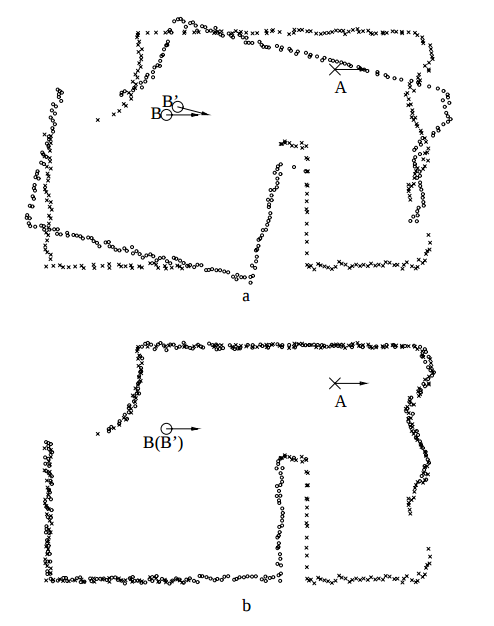
\includegraphics[width=5cm,keepaspectratio]{images/pose_estimation.png}
	\label{fig:pose_estimation}
	\caption{An example of pose registration: the robot has moved from pose A to B, but due to odometric error believes it is in B'. Points on it's current scan B' can be transformed and rotated to overlay the points obtained from a scan at B, which would allow it the robot to obtain it's current position relative to B. Source: \citet{Lu1997-zv}.}
\end{figure}
\subsection{Iterative Closest Point and variants}

The Iterative Closest Point algorithm (ICP) is one of the first, if not the fundamental starting point for the applications of heuristic algorithms to the matching of scanned data to environment maps within the context of indoor localisation.

In this point-point data representation, the algorithm first detailed by \citet{Besl1992-pd} aims to find an optimal transformation to apply to the scan which minimises the sum of the distances measured of each scan-point to their closest point in the reference map. This can be pre-processed with the removal of points with no proximate matching point, and iteratively changing the solution tuple to minimise the error using the Newton or Lorentzian methods \cite{Munoz2005-gt}. Starting from an initial position and a scan of the environment from this position, the algorithm will converge to a local optimum alignment. 

Many improvements have been suggested (20 736 variations according to \citet{Donoso2017-wp}), which aim to improve the convergence speed \cite{Donoso2017-wp} \cite{Simon1996-dl}, removal of points from the datasets which would reduce the optimality of the solution \cite{Weik1997-px} \cite{Masuda1996-av} or the precision metric used \cite{Eggert1997-ak}. As such it continues to be a strong area of research, and can prove to be an accurate and relatively quick solution to scan matching.

However, ICP finds a local optimum from a hypothetical pose: this would inhibit the algorithm from finding a global position in a single run, and this is reflected by \citet{Censi2005-iv} who states that "any 'local' matcher can be (inefficiently) used for a global search". This could be implemented by randomising the starting pose over multiple runs, highlighting the additional complexity required to adapt this algorithm into a global search.

Nevertheless it continues to be an area of continuous research, as \citet{Minguez2006-nj} developed a version of ICP in 2006 named mbICP;  this accounts for the issue that the distance of a scanned point from the sensor will be proportional to the translation error of that point due to a rotational error. This would therefore skew the error of the hypothetical translation, potentially driving it away from a local error minima.

Similarly,TrICP \cite{Chetverikov2005-yz} implements a Trimmed Least Squares \cite{Ruppert1980-js} algorithm rather than a Least Squares, improving the robustness to noise or poor initial estimations of the pose. This functions on a subset of points, thereby preventing erroneous measurements or outliers from affecting the overall regression. The algorithm is not pareto dominant to a standard ICP, as demonstrated by \citeauthor{Chetverikov2005-yz} through the examples in \autoref{fig:trICP_misalignment}; the TrICP algorithm was unable to align the M and P scans to form the correct R scan, wereas an ICP algorithm was able to achieve this result. 


\begin{figure}[t]
	\centering
	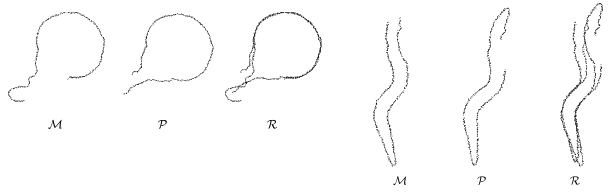
\includegraphics[width=\textwidth,keepaspectratio]{images/trICP_misalignment.png}
	\label{fig:trICP_misalignment}
	\caption{TrICP mis-alignment. Source: \citet{Chetverikov2005-yz}.}
\end{figure}

Various forms of ICP therefore out-perform each other depending on the case at hand: \citet{Donoso2017-wp} recently published a comprehensive overview of 20,736 variants of the ICP algorithm in their ability to consolidate (and therefore place relative to each other) sets of 3 sets of 100 scans at distinct locations. These variants were generated by decomposing major ICP algorithms into their components (such as their point selection criteria, neighbourhood selection, point matching, etc), and creating new algorithms using every permutation of components. He finds that the performance (precision, accuracy and computational efficiency) of ICP variants can significantly vary depending on the scan and map data, and that no single algorithm was able to adequately solve all 3 scenes in the experiment. As such, the selection of a particular variant of ICP may be significant to the effectiveness of scan matching, as we will later discuss in \ref{sec:hybrid_approaches}.


\subsection{Iterative Dual Correspondence}

The development of the IDC algorithm by \citet{Lu1997-zv} focused on the same issue in ICP for which mbICP was developed: distant points in a scan have a large matching error due to translation errors, relative to closer points. To solve this, IDC matches points in polar form. This results in a reduced computational complexity, as rather than search a 3-dimensional space, it solves an efficient one-dimensional search followed by a least squares solution. This is achieved by computing a trial value of the rotation from a global search on tangent directions from each scan, before executing a least-squares to affine the translation and rotation. This would have to be adapted for use in global localisation where the entirety of the map is not visible from a single scanning point due to range limitations, but does highlight some areas for improvement in ICP, both in terms of removing un-necessary data conversion and reducing the complexity of the algorithm. The method would also be difficult to apply to global localisation due to a lack of global search: an optimal minima would only be found if the initial error in rotation is relatively small (< 15$^o$).


\subsection{Polar Scan Matching}
\label{subsec:psm}
%TODO how to apply this to scan->map?
Polar scan matching \citet{Diosi2005-nv} utilises the same concept as IDC by adapting the ICP algorithm to use polar coordinates in an effort of minimising computational requirements. After pre-processing each scan to remove inconsistent data (due to moving objects) and segmenting the points according to a threshold criteria, the current scan is re-projected from the reference position (as demonstrated in \autoref{fig:polar_projection}, and the remaining translation and orientation is then iteratively improved. This method therefore benefits from the direct use of raw data from a laser scanner, in addition to a reduction in the dimensionality of the problem through matching the bearings of the polar data by distance. 

\begin{figure}[t]
	\centering
	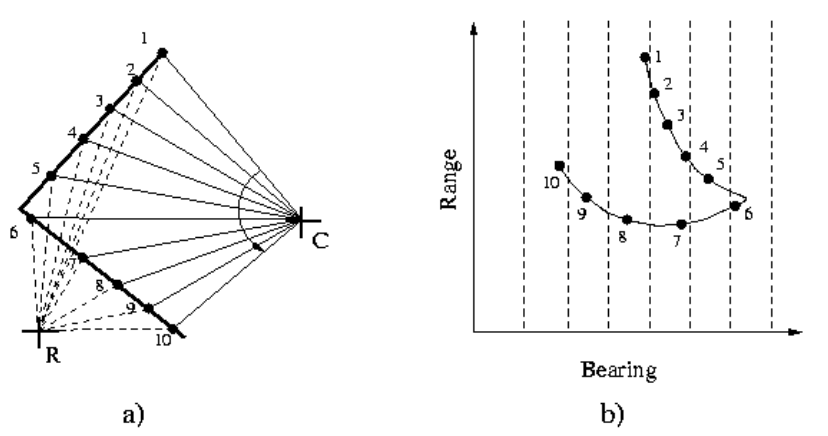
\includegraphics[width=\textwidth,keepaspectratio]{images/polar_projection.png}
	\label{fig:polar_projection}
	\caption{Polar scan projection: Points taken from location C, projected to location R. Source: \citet{Diosi2005-nv}.}
\end{figure}

\subsection{Principal Component Analysis}
Principal Component Analysis is a form of manifold learning which is applied to indoor localisation by constructing an eigenspace of the environment from a set of range scans taken in a 2D grid of the map. To avoid brute-forcing over every known scan of the environment, Principal Component Analysis is used to combine these, allowing subsequent scan matching to be done by measuring the relative similarity of the scan to points in the eigenmap, as each scan location will project to a point in the eigenspace. A nearest neighbour search in the eigenspace can then determine the most likely candidate pose. This nearest known pose can then be refined through odometric movement \cite{Pourraz1999-nu}, or by collective enough scans to provide a denser data-point matching sufficient to match a criteria of accuracy \citet{Pourraz1999-nu}. As such, the application of PCA to the method reduces to a classification problem, unless additional measures are taken to refine the solution. Additional computation, such as calculating the pose as an average of the coordinates of the $n$ nearest neighbours, could enhance this method to provide accurate global search, but this has not yet been investigated. 

\subsection{Normal distribution transform}
The normal distribution transform (NDT) by \citet{Biber2003-kb} is one of the first tangential research away from point set/feature matching. The set of points in a map can be converted into a piecewise probability density function over a 2D plane. This can be decomposed into a set of normal distributions, and the second scan can be matched by maximising the sum that the aligned points score on the previous density. The scan matching is hence performed in a different domain, using information preserving transformations. This is readily applicable to our case study, as a set of normal distributions of a map could be pre-computed, thereby avoiding repeated computations. As it relies on creating statistical approximations of the dataset, NDT requires a relatively dense data set for it's map representation; this has the side effect of making it extremely resilient to noisy data. This does remain a form of local search, in-line with previous attempts to produce an odometric correction algorithm rather than a generic localisation. The use of a novel form of hypothetical pose estimation may however be extremely viable when combined with a global search heuristic, such as a genetic algorithm [EXPLORE LATER].


\subsection{Hausdorff distance}
The usage of the Hausdorff distance was introduced by \citet{Donoso-Aguirre2008-pb}; it is defined as the maximum distance between a point in the scan and it's closest point in the map, as demonstrated in \autoref{fig:hausdorff}. As such, it signifies that every point in the scan is not any further from it's closest point in the scan than the Hausdorff distance for these sets of points. This is further improved by using the $k_{th}$ distance so as to avoid false positives due to outlying points, and instead defining the fitness function as the minimisation of the average of the first K ranked maximum Hausdorff distance. Although this could method of pose evaluation could easily be adapted into the fitness function of a genetic algorithm, the demonstrated search method would be limited to finding a local minima; without odometric data, this is unlikely to yield a global maxima. This is due to the use of an iterative gradient descent algorithm. However, the algorithm is shown to be resilient to noise and accurate when given a rough pre-alignment. Therefore, a viable adaptation of this algorithm could involve the use of coarse global search algorithm using the averaged Hausdorff as a measure of error, followed by a different algorithm to refine the roughly pre-aligned method.

\begin{figure}[t]
	\centering
	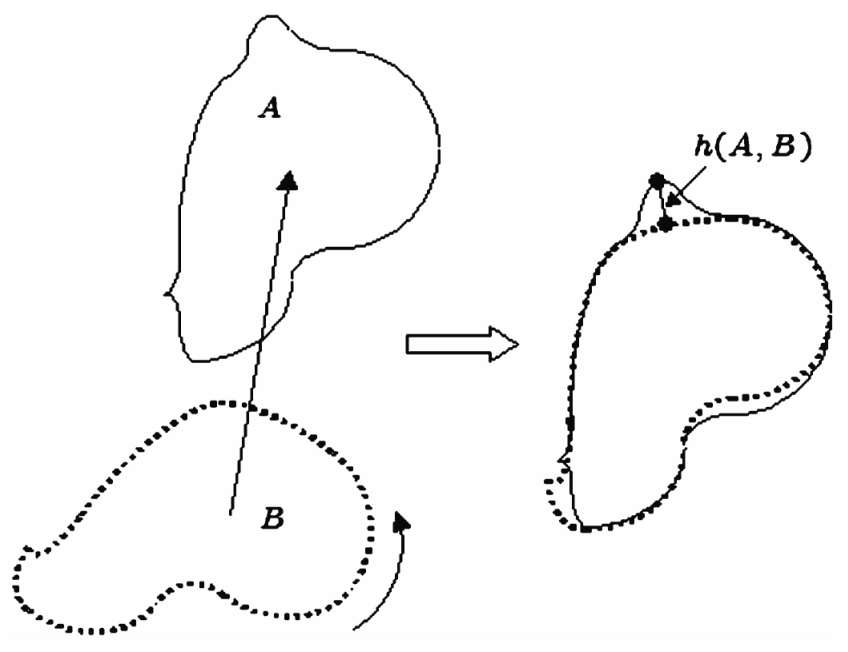
\includegraphics[width=\textwidth,keepaspectratio]{images/hausdorff.png}
	\label{fig:hausdorff}
	\caption{Hausdorff distance between points in two scans.. Source: \citet{Donoso-Aguirre2008-pb}.}
\end{figure}

\subsection{Cross-correlation scan matching}
The Cross correlation scan matching (CCSM) algorithm functions by using the set of scan points to define a 2d form, with points in the scan forming the outline of the shape. Repeating the same process using a reference scan, we obtain two equivalent shapes which we must overlay to obtain the relative pose of our robot. This is achieved by maximising the intersected area of the two shapes, as seen in \autoref{fig:cross_correlation}, where the intersected area is darkened. The method is optimised using rasterised scanning, which also helps account for sources of noise in the sensor. \citet{Konecny2016-zv} demonstrates an improved performance compared to ICP, including a higher breadth but not global search, and a significant performance improvement. No further work is conducted to evaluate it's performance on non-solid shapes (e.g: two rooms separated by a wall and door), which may impede the algorithm's effectiveness. 

\begin{figure}[t]
	\centering
	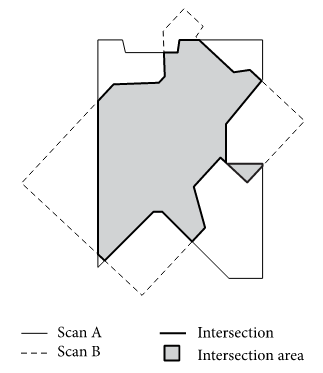
\includegraphics[width=5cm,keepaspectratio]{images/cross_correlation.png}
	\label{fig:cross_correlation}
	\caption{Matching scans by cross correlation. Source: \citet{Konecny2016-zv}.}
\end{figure}

\subsection{Hough Scan Matching}
Hough Scan Matching relies on the creation of a function which produces a spectrum from a transformed set of points (using the Hough Transform) which has the following properties; it is invariant to input translations, and is circularly shifted on the input rotation. The search is therefore performed in a different domain which was created using an information-preserving transformation. The output of the scan and map sets can then be combined using a cross-correlation operator to retrieve the relative rotation. From there, a variety of other algorithms can retrieve the most likely translation given one or more candidate rotations; the method can therefore provide a ranked output of possible pose estimations. As presented by \citet{Censi2005-iv}, hough scan matching is therefore a potent, low-complexity approach to global indoor localisation. It may be particularly adaptable to a scan-to-map application as the spectrum of the map could be pre-computed, thereby reducing the processing time for repeated pose estimations.

\subsection{Histogram scan matching}
Histogram scan matching (HSM) was first detailed by \citet{Weiss1994-ub}. It functions by creating a histogram of the range of angles between points in a scan. By building graphs of the scan and map, we can obtain two comparable histograms with some degree of phase shift matching the relative pose rotation. Aligning the two histograms using maximas and minimas would allow the retrieval of candidate rotations. The process can then be repeated using histograms of the distances between points along the x and y axis, before being matched in a similar fashion. As such, the algorithm can determine the 3-tuple pose transformation in 3 consecutive $O(n)$ operations, greatly reducing the complexity of the algorithm relative to other methods. This resulted in a global search algorithm which was tested on relatively large rotations and transitions, but lacked any comparison to other algorithms: as such it is difficult to evaluate it's relative performance. HSM can however provide a global search with a low computational cost, that is resilient to noise.

\section{Evolutionary Algorithms}
\label{sec:evo_approaches}
\subsection{Overview of genetic algorithms}
Evolutionary algorithms (EAs) are a type of meta-heuristic algorithms inspired from biological natural selection. As detailed by \citet{Whitley1994-tx}, evolutionary algorithms utilise a population of individuals, each with their own set of 'chromosomes' which would provide a solution to a given problem. These individuals are then evaluated against a stated fitness function, then selected by fitness using a competitive method which returns a 'fitter' subset of the population. This elite are then mutated to introduce a probability of improving their solution, and are crossed over with each other to share the benefits that they have inherited or mutated. This new population is then passed through the same process, and the process is repeated for a number of cycles, with each generation developing a fitter (and therefore better) solution to the given problem. 

Evolutionary algorithms therefore form an alternative to the iterative improvement strategy found in the 'classical' methods previously discussed. This divergence is notable in two ways: firstly, a large number of alternative methods used to evaluate the resultant error from a transformation/rotation tuple can be adapted into the evolutionary algorithm's fitness function, and therefore the genetic algorithm could theoretically discover equivalently optimal minima in the fitness landscape. Secondly, as the initial population can be assigned to poses distributed around the map, and the random nature of a evolutionary algorithms allow individuals to progress against a fitness gradient through mutations and cross-overs, a global optima can be found. Evolutionary algorithms therefore allow many of the previously designed algorithms to be adapted into a solution to generically locate oneself in an environment with no prior knowledge of our displacement.

The use genetic algorithms to search for data-matching was first proposed by \citet{Brunnstrom1996-vo} in \citeyear{Brunnstrom1996-vo}; this focused on the ability to find the correspondence between 2 detailed surface models. This was achieved by using a chromosome design based on a transformation, translation and rotation in 3 dimensions. As our scan matching only utilises 2-dimensional data, and temporarily ignoring the need for a transformation to handle noise, this chromosome design overcomplicates the application of scan matching in 2D indoor localisation. As such, the general chromosome design (without accounting for noise management) would simply consist of the 3-tuple previously detailed, composed of 2 transformations and a rotation.

\subsection{Parallel Evolutionary Registration of Range Data}
\citet{Robertson2002-ou} presented one of the first applications of genetic algorithms as an alternative to the ICP algorithm. Most notably, he contrasts the limitations of ICP (requiring pre-registration by hand to converge to a global minimum, tendency to converge to sub-optimal or incorrect solutions) with the benefits of a genetic algorithm; the latter does not require any form of pre-alignment, and has a significantly broader basin of convergence, allowing it to search for global solutions without any prior knowledge. This is implemented using a 3-tuple matching our problem definition, and results in significantly better global search results than a single ICP run. This therefore demonstrates the potential of genetic algorithms within the field, setting the path for following research.

\subsection{Genetic Algorithm Polar Scan matching}
Polar Scan matching (PSM) is a variation of \citeauthor{Robertson2002-ou}\'s initial genetic algorithm which is adapted for the use of raw data from a laser range scanner, and therefore benefits from a more efficient computation and a reduced search dimensionality. \citet{Ze-Su2007-li} believes this would represent two $O(n)$ searches: one for the translation estimation, and one for the orientation estimation. This approach is found by \citeauthor{Ze-Su2007-li} to be more precise and efficient than ICP in the given examples, although given the variation in performance of algorithms in scenes \cite{Donoso2017-wp} this result may not be generalisable. As demonstrated by \citeauthor{Ze-Su2007-li}, the method is applied to identify two complete sets of data, rather than mapping a subset of the data (the area visible around the robot) into the full set of data (the full map); further adaption may therefore be required for the method to function for general indoor localisation.

\subsection{Genetic Lookup based Algorithm for Scan Matching}
The Genetic Lookup based Algorithm for Scan Matching (GLASM) \cite{Lenac2007-xm} is an improvement in the efficiency of the fitness function used in a GA for indoor localisation. This is achieved by discretising the map of the environment from a set of 2D coordinates into a look-up table. A regular grid is overlayed onto the map of the environment, with individual cells marked with a boolean 1 if one or more points lie within a threshold of the grid-space, and a 0 otherwise. The fitness of a translation can then be calculated by doing a direct lookup of each scan point in the grid to establish if a map point exists near that location. The sum of these points would then be maximised to achieve a minimal error of pose alignment. As such, GLASM is one of the first algorithms which would be extremely efficient for global localisation as the lookup table could be constructed once per map and used repeatedly during each iterative improvement or run. Furthermore, the lookup table reduces the complexity required to evaluate a pose from $O(n^2)$ with point-point matching into $O(n)$ for a single lookup per scan point. However, the discretisation of the search space would lead to a decrease in accuracy due to the resolution of the lookup grid. One should also mention the additional memory required to represent such a lookup table, although \citeauthor{Lenac2007-xm} provides an example $100\times100m$ grid with a resolution of 10cm and a $125kb$ memory requirement; this is negligible considering it could easily fit into the cache of a modern Intel Core i7 processor, or the RAM of an embedded system, and would therefore not greatly hamper the performance or push the memory limitations of a system. 

\subsection{Dynamic Genetic Algorithm}
The Dynamic Genetic Algorithm by \citet{Chow2004-xc} (DGA) aims to greatly improve the accuracy of a genetic algorithm. This is achieved by repeating the algorithm in a reduced search space based off the result of previous algorithm, with a reduced step size to allow a fine-tuning of the solution. The algorithm utilises a fitness function based on minimising the sum of the distances between each point in the scan and it's closest point in the map, using a fast nearest neighbour algorithm. This search space is determined based on the range of chromosomes of a 'converged' population from the previous iteration. However, if the population converged to a sub-optimal error minima, this resulted in an affine search for a non-global minima. As this was noticed by \citeauthor{Chow2004-xc}, a random sampling from the constricted environment and far-search environment allowed a balance between exploration and exploitation. In the event of a stagnation in fitness across multiple generations, the boundary could be further constricted to increase the likelihood of an improvement through chromosome mutation. 

This would be repeated until further boundary reduction yields no improvements in fitness, leading to an optimal solution. This algorithm was found to be effective to join parts of 3D models, with a 1000 times reduction in computational time compared to a standard GA; whilst further detail is omitted, this is most likely an improvement in the convergence rate of the algorithm, allowing it to halt in fewer generations. The improvement in computational time does strongly clash with the statistical results provided in Table 1. \cite{Chow2004-xc}. Using a simple independent T-test, we can find the dynamic GA to be significantly more precise ($p<0.0001, \triangle d = 10mm$), without requiring a significantly larger number of generations ($p=0.5445$), but with a significant increase in computational time ($p<0.001, \triangle s = 40$). DGAs are therefore more precise than a standard GA (in the given test conditions, which may not be generalisable), but may be less precise than an ICP algorithm which was pre-aligned. \citet{Lomonosov2006-vq} criticised the approach's use of GAs as "faster and more precise iterative methods exist for registration of pre-aligned datasets"; as such, a hybrid algorithm such as those discussed in \ref{sec:hybrid_approaches} may produce equivalent results with less computational requirements.

\section{Hybrid approaches}
\label{sec:hybrid_approaches}
\subsection{GA \& ICP}
The concept of combining the global search of a GA with the accuracy of the ICP algorithm has been introduced in a variety of concepts. \citet{Brunnstrom1996-vo} first proposed the idea of applying a low-accuracy global search using a GA, before refining the most promising individual poses using an ICP algorithm using the pre-aligned poses. Using a fitness function defined by minimising the sum of the distance between pairs of closest points (each pair composed of a point in the scan and a point in the map), \citeauthor{Brunnstrom1996-vo} presents an objective set of results demonstrating the algorithms ability to roughly estimate the 3-tuple pose modification, but produces no statistical data regarding the success rate or precision of the algorithm. 

The hybrid approach was independently presented by \citet{Martinez2006-ci}, resulting in a method which is indistinguishable from a standard GA, but is however quicker to execute as the GA search can be completed in a coarser accuracy, thereby reducing the computational costs sufficiently in spite of the ICP execution. This utilises a fitness function similar to the PSM discussed in \ref{subsec:psm}, thereby reducing the complexity of the fitness function to $O(n)$. When compared to a standard ICP and GA, the hybrid GA-ICP method performs as well as the GA and better than ICP, with a computation time between that of an ICP and GA. Whilst the significance of these results are limited by the lack of statistical analysis and the possible lack of generalisability of localisation algorithms, it is difficult to demonstrate this hybrid approach to be superior to other available methods. As such, further evaluation of the GA-ICP algorithm in a larger variety of environments would be required to find the strengths and weaknesses of the approach relative to differing environments. One should note these papers used a basic form of ICP, and as such were quickly improved upon as discussed below.


\subsection{GA \& TrICP}
\citet{Lomonosov2006-vq} presents a comparative analysis of a new algorithm; a combination of a genetic algorithm with the refined, precise and robust TrICP. As with \cite{Brunnstrom1996-vo} and \cite{Martinez2006-ci}, the algorithm executes a coarse GA search for candidate poses, before refining the most promising pose using TrICP. This allows the construction of a global search algorithm with a claimed higher precision than a GA, which was effectively applied to merge sections of 3D models. As such, it could be effectively applied to our problem, but is not compared to a standard GA in terms of computational requirements or precision. 

\subsection{Hybrid Genetic Lookup based Algorithm}
The Hybrid Genetic Lookup based Algorithm for Scan Matching (h-GLASM) by \citet{Lenac2011-co} is a combination of the mbICP algorithm with the fast lookup genetic algorithm. This aims to benefit from the global search provided by a genetic algorithm, the improvement in performance attained by the GLASM algorithm, and improve the accuracy of the final solution by executing an mbICP algorithm on a maximally pre-aligned pose. This results in a rapid, global search which is capable of producing an equal or higher success rate than a standard mbICP, but the precision of this algorithm is not evaluated or compared to other algorithms in the scope of it's paper. As such it is difficult to consider it's accuracy, although we could hypothesise that it is capable of a global search comparable to the GLASM algorithm, with the precision of the mbICP algorithm; this would make it the ideal starting point for further development of an indoor localisation system based on the use of a laser scanner and no prior pose information.

\section{Summary}
These paradigms illustrate the breadth of research in the area of indoor localisation. 'Classical' methods (ICP, IDP, classical PSM, PCA) continue to be developed and improved, resulting in algorithms which can quickly and accurately enhance odometric data, but generally lack a form of global search. Other classical methods search a modified space (PCA, Hough Scan Matching, Histogram Scan Matching), allowing them to produce global results, but their accuracy is rarely compared to local classical methods; this is due to the purpose of these algorithms, which is to locate oneself a global environment, rather than correct an existing pose. As such, a majority of these classical algorithms are unsuitable for localising a robot without any prior knowledge of the robot's pose.

The third paradigm involves using the searching potential of a genetic algorithm in combination with a fitness function mimicking the error function used in classical methods, providing a global search over the map. However, these are unable to produce equally accurate results in comparison to classical methods, leading to the development of hybrid algorithms. As these provide the accuracy of a 'classical' method with the global search of a genetic algorithm, they are most suitable to the problem of global localisation in a known environment but no prior pose information. 

Developments in this area continue to integrate new classical methods (TrICP or mbICP) to improve the accuracy of the fine-tuning, or focus on optimising the performance of the genetic algorithm (GLASM). This leads us to the following question: are there any better classical methods (e.g: Hausdorff distance) which could be integrated with a genetic algorithm to improve upon the H-GLASM or GA-ICP algorithms? How do these methods compare with classical search algorithms such as the Hough or Histogram scan matching?

\cleardoublepage

\bibliographystyle{unsrt}
\bibliography{references}

\end{document}
